%!TEX root = ../thesis.tex
\chapter{Objekterkennung mit neuronalen Netzen}
\label{ch:Theoretischer Hintergrund}



{
	\begin{figure}[ht]
        \centering
		\begin{subfigure}[b]{0.45\textwidth}
            \centering
            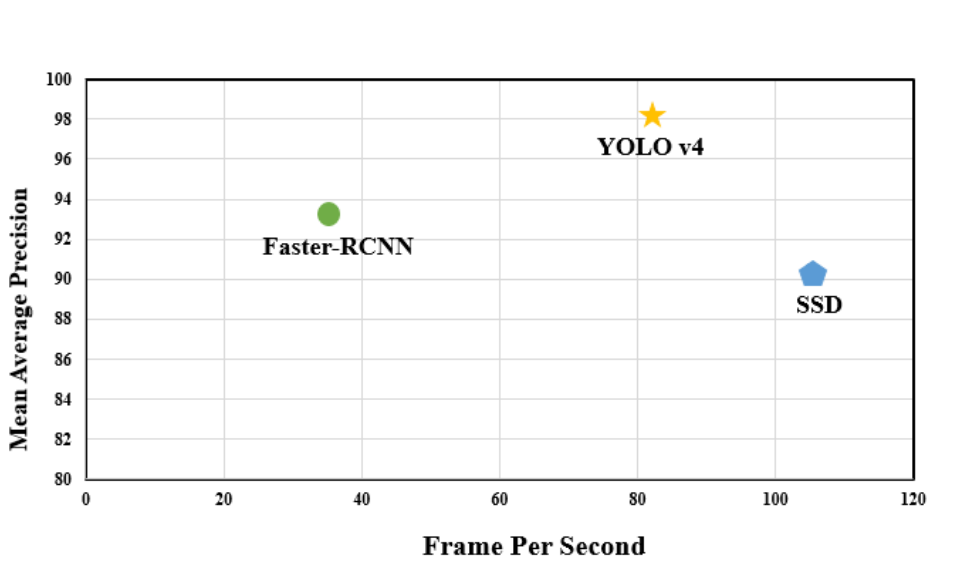
\includegraphics[width=\linewidth]{images/yolo_comp/Yolo_ssd_fRCNN.png}
            \caption[Performance von verschiedenen Objektdetektoren]{Performance von verschiedenen Objektdetektoren  \cite{Kim2020_2}}
            \label{Scr:Perf_ObDet}
        \end{subfigure} 
		\hfill
		\begin{subfigure}[b]{0.50\textwidth}
			\begin{tabular}{l|l|l|l} 	
			 & \textbf{YOLO\_v4} & \textbf{SSD} & \textbf{Faster-RCNN} \\ \hline
			\textit{FPS} & 82,1 & 105,14 & 36,32 \\ \hline
			\textit{F1Score} & 0,96 & 0,88 & 0,90 \\ \hline
			\textit{Precision} & 0,93 & 0,90 & 0,86 \\ \hline
			\textit{Recall} & 0,98 & 0,87 & 0,94 \\ \hline
			\textit{mAP} & 98,19 & 90,56 & 93,40
			\end{tabular}
			\vspace{0,65cm}
			\caption[Vergleichswerte verschiedener Objektdetektoren]{Vergleichswerte verschiedener Objektdetektoren (GPU: GeForce RTX2080Ti) \citep{Kim2020_2}}
			\label{tab:comp_Objdetect}
	\end{subfigure}      
        \caption[Vergleich von verschiedenen Objektdetektionsalgorithmen (YOLO, SSD, F-RCNN)]{Vergleich von verschiedenen Objektdetektionsalgorithmen (YOLO, SSD, F-RCNN) \cite{Kim2020_2}}
        %\label{Scr:comp_object_detector}
    \end{figure}
	
Im Folgenden wird sich hauptsächlich auf Objektdetektion auf Bildern bezogen, weil Videos aus einzelnen schnell aufeinander folgenden Bildern (auch Frames genannt) bestehen. \\
Zur Objekterkennung auf Bildern gibt es verschiedene Möglichkeiten. Es gibt ressourcenschonende Ansätze, wie die Schwellwertsegmentierung nach \citeauthor{Otsu1979} \cite{Otsu1979}. Dieses Segmentierungsverfahren ist zwar sehr schnell, nimmt aber keine Klassifikation der segmentierten Objekte vor, wodurch eine Nutzung im Rahmen dieser Arbeit als nicht sinnvoll erachtet wird. Dadurch, dass keine Klassifikation vorgenommen wird, kann nicht zwischen irrelevanten und relevanten Objektumrissen unterschieden werden. \\
Maschinelles Lernen kann die Herausforderung der gleichzeitigen Objektdetektion mit entsprechender Klassifizierung lösen. Eine weitere Herausforderung, dass Detektion von Fahrzeugen immer aufwendiger wird, da der Verkehr heterogener wird, ähnelt dieser Arbeit, da der Erfolg von Verkehrstracking von der Genauigkeit und Performance der verwendeten Algorithmen abhängt \citep{Pavani2022}. Außerdem muss die Fahrzeugdetektion schnell und sicher sein, da das Fahrzeug richtig klassifiziert werden muss, während es sich auf der Straße bewegt \citep{Kim2020_2}. \\
Hierzu existieren verschiedene Algorithmen, wie CNN (\glqq Convolutional Neural Network\grqq{}), KNN (\glqq k-nearest neighbors\grqq{} Algorithmus), den SSD (\glqq Single Shot Detector\grqq), den Haarcascade Algorithmus oder \glqq You Only Look Once\grqq{} (YOLO) \citep{Pavani2022, Kim2020_2}. \\
Von \citeauthor{Kim2020_2} \cite{Kim2020_2} wurde ein Vergleich zwischen YOLOv4, dem SSD Algorithmus und dem Faster-RCNN Algorithmus zur Echtzeitdetektion von Fahrzeugtypen vorgestellt \citep{Kim2020_2}. Für einen Vergleich der anderen genannten Algorithmen s. Abb. \ref{scr:comp_obj_det_mean_av} (S. \pageref{scr:comp_obj_det_mean_av}) und \ref{Scr:comp_object_detector} (S. \pageref{Scr:comp_object_detector}) \citep{Pavani2022}. \\
Wenn man die Präzision und Genauigkeit (s. \ref{tab:comp_Objdetect}) von den verschiedenen Algorithmen vergleicht, ist zu erkennen, dass YOLO die höchste Präzision besitzt. Außerdem kann YOLO die beste mAP (Mean Average Precision) (s. \ref{Scr:Perf_ObDet}) bei gleichzeitig hohen FPS vorweisen.  Dies liegt an der neuartigen Implementierung von YOLO, die im Folgenden näher erläutert wird. \\
Der YOLO Algorithmus wird aus den genannten Gründen in dieser Arbeit verwendet und es wird zunächst kurz auf die Grundlagen des YOLO Algorithmus eingegangen.

 }


%\section{\glqq You Only Look Once\grqq{}(YOLO)}
{ 
	
	\section{Der YOLO Algorithmus \label{subsec:YOLO_Alg}} 
	{Da der Blick des Menschen Objekterkennung, -einordnung und -wirkung intuitiv ermöglicht, ist es unserem Gehirn im Zusammenspiel mit unseren Augen möglich, schnell und genau zu sehen. Durch diese Fähigkeiten können wir mit nur wenig bewussten Gedanken komplexe Aufgaben, wie Fahrradfahren bewältigen, bei denen gleichzeitig mehrere Sinne beansprucht werden. \citep{Redmon2016}. \\
	Dem Computer kann dies mit schnellen und genauen Algorithmen zur Objekterkennung beigebracht werden. Aktuelle Systeme nutzen Klassifikatoren zur Objekterkennung. Dieser wird an verschiedenen Stellen in variablen Skalierungen im Testbild angewendet, um eine Klassifizierung eines Objektes zu ermöglichen \citep{Redmon2016}. \\ 
	
	\begin{figure}[ht]
		\centering
		\includegraphics*[scale = 1, keepaspectratio, trim=2 2 2 2 ]{images/YOLO/YOLO_detection_system.png}
		\caption[Das YOLO Objekterkennungsystem]{Das YOLO Objekterkennungsystem \citep{Redmon2016}}
		\label{YOLO_Objectdetection}
 	\end{figure}\glqq You Only Look Once\grqq{} (YOLO) betrachtet Objekterkennung als einzelnes Regressionsproblem, indem direkt von Bildpixel zu Boundingbox Koordinaten und Klassenwahrscheinlichkeiten berechnet wird. Dieser Algorithmus analysiert nur einmal ein Bild und sagt direkt vorher, welche Objekte wo vorhanden sind. Dadurch ist die Komplexität des  Aufbaus von YOLO sehr gering, wie in Abb. \ref{YOLO_Objectdetection} zu sehen \citep{Redmon2016}. \\
	Die Performance zur Objekterkennung wird durch das Training von YOLO mit vollständigen Bildern gesteigert. Durch dieses vereinheitlichte Modell entstehen mehrere Vorteile gegenüber den traditionellen Objekterkennungssystemen \citep{Redmon2016}. \\
	Der erste Vorteil von YOLO ist die gesteigerte Performance. Dies wird dadurch ermöglicht, dass Objekterkennung auf Bildern als Regressionproblem betrachtet wird und deshalb keine komplexe Pipeline die Verarbeitung eines Bildes verlangsamt.  \citep{Redmon2016}. 
	Zweitens analysiert YOLO ein Bild global mit Vorhersagen zur Objekterkennung. Dadurch kann YOLO den Fehler beim Verwechseln von Hintergrund und Objekten im Vordergrund um die Hälfte im Vergleich zu Fast R-CNN verringern. Dies geschieht vor allem durch den größeren Kontext, den YOLO durch die Gesamtbildanalyse gewinnt \citep{Redmon2016}. \\
	Der dritte Vorteil ist das YOLO mit generalisierten Repräsentationen von Objekten trainiert wurde um die Fehlertoleranz bei der Anwendung auf neue Bereiche und unerwartete Eingaben zu vergrößern, aufgrund der Möglichkeit der hohen Verallgemeinerung \citep{Redmon2016}. \\
	Ein Nachteil von YOLO liegt in der Genauigkeit. Der Algorithmus hat Schwierigkeiten einige, insbesondere kleine, Objekte genau zu lokalisieren \citep{Redmon2016}. \\
	Da der Quellcode, mehrere vortrainierte Modelle und die Trainingsdaten von YOLO Open-Source sind und zum Download bereitstehen, ist dieser Algorithmus für den Rahmen dieser Arbeit leicht zugänglich und anwendbar \citep{Redmon2016}. \\

	YOLO unterteilt in Bild in $S \times S $ Rasterzellen. Wenn der Mittelpunkt eines Objektes in eine Rasterzelle fällt, ist diese für die Erkennung des Objektes zuständig. Boundingboxen und ihre jeweiligen Confidence Scores werden für jede Rasterzelle vorhergesagt \citep{Redmon2016}.
	Der Confidence Score beschreibt, wie sicher sich das Modell ist, dass die Boundingbox ein Objekt dieser Klasse enthält und für wie genau das Modell diese Vorhersage hält. \\
	Dieser Wert enthält nicht nur die Wahrscheinlichkeit, dass diese Klasse in der Boundingbox vorkommt, sondern auch wie gut die vorhergesagte Box mit dem detektierten Objekt übereinstimmt. Ein Beispielablauf ist in Abb. \ref{YOLO_Model} zu sehen.
	\begin{figure}[ht]
		\centering
		\includegraphics*[scale = 2, keepaspectratio, trim=2 2 2 2 ]{images/YOLO/YOLO_model.png}
		\caption[Das YOLO Modell]{Das YOLO Modell\citep{Redmon2016}}
		\label{YOLO_Model}
 	\end{figure}

	


	Da jede Rasterzelle nur 2 Boundingboxenvorhersagen und eine Klasse haben kann, unterliegt YOLO einer räumlichen Einschränkung. Dies begrenzt die Anzahl der benachbarten Objekte, die das Modell vorhersagen kann. Außerdem ist es für das Modell schwierig, kleine Objekte, die in Gruppen auftreten, zu detektieren \citep{Redmon2016}. \\
	Eine weitere Herausforderung ist, dass Objekte mit neuen oder ungewöhnlichen Formen auftreten können und dadurch die Vorhersage erschwert wird. Da die Netzwerkarchitektur aus mehreren \glqq Downsampling\grqq{}-Schichten besteht, benutzt das Modell relativ grobe Features zur Vorhersage der Boundingboxen \citep{Redmon2016}. \\
	Außerdem sorgt das Training mit der YOLO spezifischen Verlustfunktion (für eine Erklärung s.  Formel \ref{YOLO_Loss_function}, S. \pageref{YOLO_Loss_function} und Abb.  \ref{YOLO_loss_function_detail}, S. \pageref{YOLO_loss_function_detail}), die die Erkennungsleistung annähert, dafür dass Fehler bei kleinen Boundingboxen genauso wie bei großen Boundingboxen behandelt werden. Dies ist ein Nachteil, weil ein kleiner Fehler in einer großen Boundingbox meistens wenig Auswirkungen hat, aber ein kleiner Fehler in einer kleinen Boundingbox eine sehr viel größer Auswirkung auf die IOU hat. Falsche Lokalisierungen sind eine weitere Hauptfehlerquelle \citep{Redmon2016}. \\
	YOLO ist für den Anwendungszweck dieser Arbeit geeignet, weil der Algorithmus die entsprechende Performance und einfache Verfügbarkeit von trainierten Modellen bietet. Außerdem existieren mehrere weitere Versionen (s. Abb. \ref{YOLO_timeline_vers}, S. \pageref{YOLO_timeline_vers}) von YOLO, die Vorteile in einzelnen Aspekten bieten \citep{Terven2023}. 

	Im Rahmen dieser Arbeit wird YOLOv8 von Ultralytics verwendet. Diese bietet Vorteile in der Performance und Genauigkeit der Objektdetektierung und wird im nächsten Kapitel genauer erläutert. 
	} 

	\section{YOLOv8 von Ultralytics}{ \label{subsec:YOLOv8_theoretic}
	
	Im Januar 2023 wurde von der Firma Ultralytics YOLOv8 veröffentlicht, welches auf YOLOv5 basiert. Diese Version beinhaltet 5 verschiedene Modelle (YOLOv8n (nano), YOLOv8s (small), YOLOv8m (medium), YOLOv8l (large), YOLOv8x (extra large)), die mit unterschiedlich großen Datensätzen trainiert wurden  \citep{Terven2023}. \\	
	Ein Vorteil dieser YOLO Implementierung ist, dass verschiedene Varianten für Ob\-jekt\-det\-ekt\-ion, -seg\-men\-tier\-ung und -ver\-fol\-gung, sowie -klas\-si\-fi\-zier\-ung existieren. In dieser Arbeit wird hauptsächlich die \glqq -seg\grqq{}-Variante verwendet, welches bereits eine Segmentierung der Umrisse der detektierten Objekte integriert hat.
	\begin{figure}[h]
		\centering
		\includegraphics*[scale = 0.20, keepaspectratio]{images/YOLO/YOLOv8_object_detector_general.png}
		\caption[Architektur modernen Objektdetektoren]{Architektur modernen Objektdetektoren \citep{Terven2023}}
		\label{YOLO_obj_det_gen}
	\end{figure}
	Die Architektur dieser Algorithmen kann man in 3 Teile aufteilen (s. Abb. \ref{YOLO_obj_det_gen}). Diese sind der Backbone, der Neck und der Head \citep{Terven2023}. \\
	Das Detektieren nützlicher Features vom Eingabebild geschieht im Backbone, welcher meist als CNN implementiert ist \citep{Terven2023}. \\
	Zwischen Backbone und Head wird der Neck eingesetzt, um die Features, die der Backbone ausgibt, zu aggregieren und zu verfeinern. Der Fokus liegt auf der Verbesserung der räumlichen und semantischen Informationen über die unterschiedlichen Skalierungen hinweg \citep{Terven2023}. \\
	Die letzte Komponente ist der Head, welcher die Vorhersagen, aufgrund der von dem Backbone und Neck gelieferten Features, trifft. Hier werden meistens aufgabenspezifische Teilnetze eingesetzt, um Klassifizierung, Lokalisierung und auch sofortige Segmentierung durchzuführen. Aus den Features, die der Neck liefert, erstellt der Head Vorhersagen für jeden Objektkandidaten. Ein Post-Procressing Schritt, wie die Non-Maximum-Supression (NMS), filtert überlappende Vorhersagen heraus, sodass nur die sichersten Detektionen genutzt werden \citep{Terven2023}.\\
	Da YOLOv8 auf YOLOv5 basiert, wird in diesem ein ähnlicher Backbone genutzt. Für die Architektur von YOLOv8 s. Abb. \ref{YOLOv8_Arch} (S. \pageref{YOLOv8_Arch}). 

	Um die Performance insbesondere bei der Objekterkennung von kleineren Objekten zu verbessern, nutzt YOLOv8 CloU \citep{Zheng2020} und DFL \citep{Li2020} Verlustfunktionen für Boundingboxloss und binäre Kreuzentropie für den Klassifizierungsloss \citep{Terven2023}. \\

	Mit dem YOLOv8-seg Modell wird auch eine Variante angeboten, die semantische Segmentierung ermöglicht. Dieses Modell wird in dieser Arbeit genutzt, da es den Anforderungen an Präzision und Performance entspricht. An den Einstellungen des YOLO-Modells, wie bspw. den Werten des Ausgabetensors, wird nichts geändert. Es werden die von Ultralytics vorgegebenen Standardeinstellungen und Modelle genutzt.
	}
}
